\documentclass[aps,prd,reprint,onecolumn,11pt,nofootinbib,notitlepage]{revtex4-2}
\usepackage[T1]{fontenc}
\usepackage[utf8]{inputenc}
\usepackage{amsmath,amssymb,bm,graphicx}
\setlength{\emergencystretch}{4em}
\usepackage[colorlinks=true,citecolor=blue,linkcolor=blue,urlcolor=blue]{hyperref}
\begin{document}
\title{Sharp quadrupole--octupole chirality and the nonlinear local distance response}
\author{Anonymous review draft}\noaffiliation

\begin{abstract}

An angular observable can contain an octupole even when its underlying local rate contains only a dipole and a quadrupole. We show how the logarithm of the directional distance law generates this coupling, and identify the tensor operator that controls its geometry. For real symmetric trace-free tensors \(Q\) and \(O\) of ranks two and three, the contraction \(v=O:Q\) fills a solid ellipsoid at fixed octupole norm. Its minimum-norm lift yields the attained maximum of the pseudoscalar \(\chi=\det[v,Qv,Q^2v]\), and optimization over quadrupole shape gives the sharp inequality \(|\chi|\le(4\sqrt2/135)\|Q\|_F^6\|O\|_F^3\). We give its equality cases, both signs, and the complete fixed-norm fibres, including zero and repeated-spectrum sectors. The same lift generates the leading acceleration--shear contribution to the local magnitude octupole. A finite logarithmic remainder bounds its four-component residual and the error of a constructive acceleration inverse. An explicit positive local-response family approaches both sharp chirality endpoints as its amplitude tends to zero. The complete ideal magnitude field also determines the dimensionless dipole and shear independently of an additive intercept. Retained spherical quadratures illustrate the quadratic coupled response, its cubic pure-dipole limit and the analytic remainder envelope.

\end{abstract}
\maketitle
\section{Introduction}

Directional observations retain more information than their multipole powers. A quadrupole supplies principal directions and eigenvalue shape; an octupole carries a relative orientation and components that cannot be reconstructed from one preferred axis. Their joint geometry can therefore matter even when their scalar powers are fixed. Multipole-vector constructions provide a familiar representation of this information \cite{Copi2004}, while harmonic-tensor invariant theory and tensor-moment pseudoscalars supply a broader mathematical setting \cite{Olive2014,Desmorat2021,Pisanty2026}.

We study the contraction of an octupole with a quadrupole. Repeated application of the quadrupole to this vector gives three vectors whose oriented volume measures one aspect of the pair's handedness. The resulting quantity has a useful optimization problem: at prescribed tensor norms, which contractions and oriented volumes are actually attained? Solving that problem gives a bounded shape coordinate, together with the tensor components it leaves unresolved.

There is a local optical use of the same construction. The directional redshift--distance slope of a smooth congruence contains expansion, acceleration and shear. The logarithm entering a distance modulus mixes their angular components. Its acceleration--shear product generates an octupole whose three-dimensional image is exactly the adjoint image of the algebraic contraction. We derive this relation in one source and observer congruence, following the local distance expansion of Kristian and Sachs and Heinesen \cite{KristianSachs1966,Heinesen2021}. The response considered here is the nonlinear conversion of a distance to a magnitude. Changing the physical observer introduces the additional transformations studied in covariant cosmography \cite{Maartens2024}.

The argument proceeds from the exact tensor image to its sharp oriented-volume bound, and then to the optical response and inverse. The geometric statements are deterministic. The numerical illustration evaluates a specified local response and supplies no sampling distribution for an observed sky.

\section{Tensor conventions and the contraction image}

Let \(Q\in\mathrm{STF}_2(\mathbb R^3)\) and \(O\in\mathrm{STF}_3(\mathbb R^3)\) be real tensors in an oriented Euclidean space. A colon contracts all displayed paired indices. Norms are full ordered-index Frobenius norms, so repeated off-diagonal entries retain their multiplicities. In particular,

\begin{equation}
 \|Q\|_F^2=\sum_iQ_{ii}^2+2\sum_{i<j}Q_{ij}^2,\qquad
 \|O\|_F^2=\sum_iO_{iii}^2+3\sum_{i\ne j}O_{iij}^2+6O_{123}^2.
 \tag{1}
\end{equation}

We write

\begin{equation}
 t=Q:Q,\quad j=\operatorname{tr}(Q^3),\quad o=\|O\|_F,\qquad
 C_QO=O:Q=v,\qquad \chi(Q,O)=\det[v,Qv,Q^2v].
 \tag{2}
\end{equation}

If the amplitudes of \(Q\) and \(O\) have units \(q\) and \(u\), then \(v\) has units \(qu\) and \(\chi\) has units \(q^6u^3\). Under a common orthogonal transformation \(R\), the contraction transforms as a vector and \(\chi\) transforms by \(\det R\). It is invariant under proper rotations and odd under reflection. A nonzero value consequently distinguishes a pair from its mirror under proper rotations. A zero value does not classify the complete tensor pair.

\textbf{Theorem 1 (attained contraction image).} For \(Q\ne0\), define

\begin{equation}
 M_Q=\frac t3 I+\frac25Q^2.
 \tag{3}
\end{equation}

The image of the sphere \(\|O\|_F=o\), \(o\ge0\), under \(C_Q\) is exactly

\begin{equation}
 \mathcal E_{Q,o}=\{v:v^{\mathsf T}M_Q^{-1}v\le o^2\}.
 \tag{4}
\end{equation}

Let \(L_Q=C_Q^*\). The fibre above \(v\) consists of

\begin{equation}
 O=L_QM_Q^{-1}v+K,\qquad K\in\ker C_Q,\qquad
 \|K\|_F^2=o^2-v^{\mathsf T}M_Q^{-1}v.
 \tag{5}
\end{equation}

The kernel is four dimensional. For \(o>0\), a fibre is a translated three-sphere at an interior point, a singleton on the boundary, and empty outside the ellipsoid. At \(o=0\), its only nonempty fibre is \(\{0\}\). At \(Q=0\), the image is \(\{0\}\), the kernel is all of \(\mathrm{STF}_3\), and the nonempty fixed-norm fibre is a six-sphere when \(o>0\).

\emph{Proof.} The adjoint is

\begin{equation}
 (L_Qw)_{ijk}
 =\frac{w_iQ_{jk}+w_jQ_{ik}+w_kQ_{ij}}3
 -\frac2{15}\left[\delta_{ij}(Qw)_k+
 \delta_{ik}(Qw)_j+\delta_{jk}(Qw)_i\right].
 \tag{6}
\end{equation}

The trace of the first term is \(2Qw/3\), and that of the bracket is \(5Qw\), so \(L_Qw\) is trace free. Contracting it with an STF tensor \(O\) removes the Kronecker terms and gives \(w\cdot C_QO\). A further contraction with \(Q\) yields

\begin{equation}
 C_QL_Qw=\frac t3w+\left(\frac23-\frac4{15}\right)Q^2w=M_Qw.
 \tag{7}
\end{equation}

Since \(M_Q\succeq(t/3)I>0\), \(C_Q\) is onto and its kernel has dimension \(7-3=4\). Its minimum-norm lift of \(v\) is \(O_0=L_QM_Q^{-1}v\). Every other lift differs by a kernel element, orthogonal to \(O_0\), whence

\begin{equation}
 \|O_0+K\|_F^2=v^{\mathsf T}M_Q^{-1}v+\|K\|_F^2.
 \tag{8}
\end{equation}

This proves necessity of (4). Conversely, every vector satisfying (4) can be lifted to norm \(o\) by assigning the residual squared norm to any direction in the kernel. Equation (5) and all stated fibre cases follow. The zero-\(Q\) case follows directly from \(C_0=0\). \(\Box\)

Without the norm constraint, the fibre is a four-dimensional affine space. Intersecting it with the norm sphere produces the three-sphere in Theorem 1. This distinction explains why a fixed-norm tensor sphere can have a solid three-dimensional image. The construction is rotation covariant: \(M_{RQR^{\mathsf T}}=RM_QR^{\mathsf T}\), and common rotation carries each fibre to the fibre above \(Rv\). At fixed \(Q\), only its stabilizer acts without changing that quadrupole.

\section{The sharp chirality bound}

\textbf{Theorem 2 (fixed-shape and global extrema).} Let \(\lambda_i\) be the eigenvalues of \(Q\), and put \(V=\prod_{i<j}(\lambda_j-\lambda_i)\). For \(Q\ne0\),

\begin{equation}
 \max_{\|O\|_F=o}|\chi(Q,O)|
 =\frac{|V|\sqrt{\det M_Q}}{3\sqrt3}\,o^3.
 \tag{9}
\end{equation}

For arbitrary \(Q,O\),

\begin{equation}
 \boxed{\ |\chi(Q,O)|\le\frac{4\sqrt2}{135}\|Q\|_F^6\|O\|_F^3.\ }
 \tag{10}
\end{equation}

For a simple spectrum and \(o>0\), equality in (9) occurs precisely at the eight contractions

\begin{equation}
 v_i=\varepsilon_i\,o\sqrt{m_i/3},\qquad
 m_i=t/3+2\lambda_i^2/5,\qquad \varepsilon_i\in\{-1,1\},
 \tag{11}
\end{equation}

with their unique boundary lifts \(O=L_QM_Q^{-1}v\). Four choices attain each sign. Nontrivial equality in (10) additionally requires \(j=0\), equivalently the spectrum \((-\sqrt{t/2},0,\sqrt{t/2})\) up to permutation. For repeated eigenvalues, \(\chi=0\) for every \(O\), so every fixed-norm octupole attains the zero maximum in (9). If either tensor is zero, both sides of (10) vanish.

\emph{Proof.} Choose a positively oriented orthonormal eigenframe. Factoring the three components of \(v\) from the determinant gives

\begin{equation}
 \chi=Vv_1v_2v_3.
 \tag{12}
\end{equation}

Write \(y_i=v_i/\sqrt{m_i}\). Theorem 1 gives \(\sum_i y_i^2\le o^2\). The arithmetic--geometric mean inequality applied to their squares gives \(|y_1y_2y_3|\le o^3/(3\sqrt3)\), with equality exactly when \(|y_i|=o/\sqrt3\). This exhausts the ellipsoid radius, and (8) forces \(K=0\). Thus the bound and all simple-spectrum equality cases in (9) are attained. When \(V=0\), (12) proves the repeated-spectrum statement directly.

To optimize the shape, trace freedom gives the characteristic polynomial

\begin{equation}
 \det(sI-Q)=s^3-\frac t2s-\frac j3.
 \tag{13}
\end{equation}

Its discriminant and elementary symmetric functions give

\begin{equation}
 V^2=\frac{t^3}{2}-3j^2,\qquad
 \det M_Q=\frac{64t^3}{675}+\frac{8j^2}{1125},\qquad
 0\le r:=\frac{j^2}{t^3}\le\frac16.
 \tag{14}
\end{equation}

For completeness, \(\sum_{i<j}\lambda_i^2\lambda_j^2=t^2/4\) and \(\prod_i\lambda_i^2=j^2/9\); expanding \(\prod_i(t/3+2\lambda_i^2/5)\) proves the middle identity. After removing \(t^6o^6/27\) from the squared bound in (9), the remaining factor is

\begin{equation}
 p(r)=\left(\frac12-3r\right)
       \left(\frac{64}{675}+\frac{8r}{1125}\right),\qquad
 p'(r)=-\frac{316+48r}{1125}<0.
 \tag{15}
\end{equation}

The maximum therefore occurs at \(j=0\). Substitution gives (10). A unit-norm witness is

\begin{equation}
 Q_* =\operatorname{diag}(-1/\sqrt2,0,1/\sqrt2),\qquad
 w_*=(\sqrt{10}/4,1,\sqrt{10}/4),\qquad O_*=L_{Q_*}w_*.
 \tag{16}
\end{equation}

Here \(M_{Q_*}=\operatorname{diag}(8/15,1/3,8/15)\), so \(\|O_*\|_F^2=w_*^{\mathsf T}M_{Q_*}w_*=1\). Its contraction is \((2\sqrt{10}/15,1/3,2\sqrt{10}/15)\), and (12) gives \(\chi=4\sqrt2/135\). Replacing \(O_*\) by \(-O_*\), or reflecting the pair, gives the negative endpoint. \(\Box\)

For nonzero \(Q\) and \(O\), define the dimensionless coordinate

\begin{equation}
 \mathcal C=\frac{135\chi}{4\sqrt2\,t^3o^3},\qquad
 |\mathcal C|\le E(r):=\sqrt{(1-6r)(1+3r/40)}\le1.
 \tag{17}
\end{equation}

The global endpoints occur at \(r=0\), and repeated spectra give \(r=1/6\) and \(\mathcal C=0\). The ratio \(|\mathcal C|/E(r)\) is defined only for simple spectra. Neither normalized ratio is assigned a value at a zero tensor. The polynomial and its unnormalized bound remain defined there. Positive amplitude rescaling cancels from \(\mathcal C\), consistently with \(\chi(aQ,bO)=a^6b^3\chi(Q,O)\).

For a simple diagonal quadrupole, its proper-rotation stabilizer consists of diagonal sign matrices of determinant one. These connect the four extrema with each product sign in (11). Thus the eight boundary lifts form two proper-rotation classes at fixed \(Q\). Figure~\ref{fig:geometry} shows their contraction geometry and the shape envelope; Figure~\ref{fig:extremizer} displays an extremal pair and its mirror.


\begin{figure}[htb]\centering
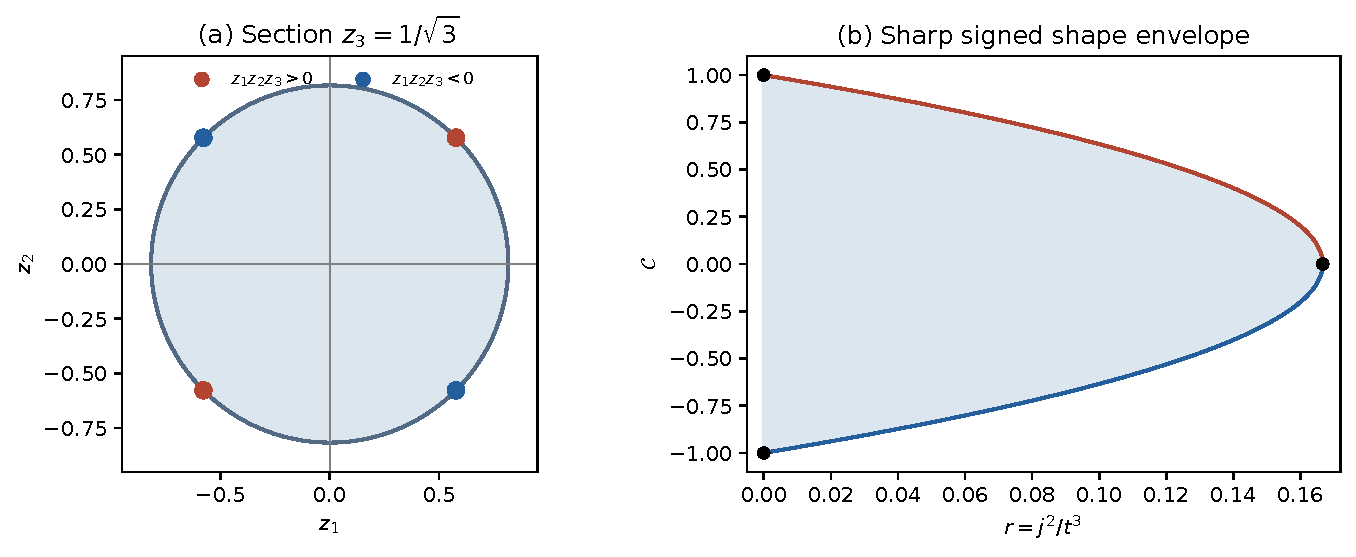
\includegraphics[width=\linewidth]{figures/geometry.pdf}
\caption{Attained contraction geometry. At fixed quadrupole and octupole norm the normalized contraction vector fills the unit ball. The displayed section contains four of the eight simple-spectrum extremizers; the remaining four lie in the opposite section. The fixed-norm fibre is a translated three-sphere in the interior and a singleton on the boundary. The right panel shows the sharp signed shape envelope, which reaches both global endpoints at a zero-cubic-trace quadrupole and vanishes at repeated eigenvalues. The coordinates are dimensionless analytic quantities, not sample probabilities.}\label{fig:geometry}
\end{figure}

\begin{figure}[htb]\centering
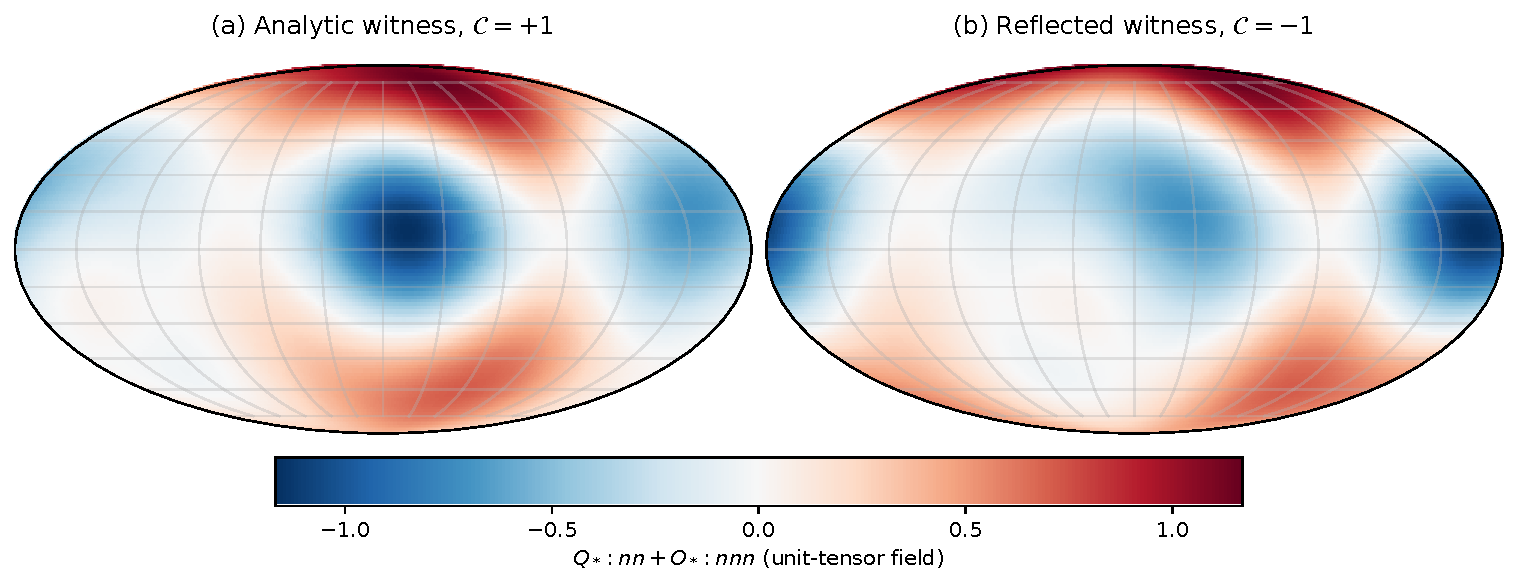
\includegraphics[width=\linewidth]{figures/extremizer.pdf}
\caption{An analytic pair attaining the sharp constant and its mirror. Both STF tensors have unit Frobenius norm. Reflection preserves their norms and reverses the determinant coordinate. The fields illustrate the algebraic theorem; the exact logarithmic optical response has its separately stated amplitude and remainder restrictions. These unit-tensor angular fields are synthetic illustrations in the specified common Euclidean frame.}\label{fig:extremizer}
\end{figure}
\subsection{Relation to a conventional tensor covariant}

The spectral factor in (14) is the discriminant appearing in harmonic-tensor invariant theory \cite{Desmorat2021}. To fix the cross-product convention explicitly, define

\begin{equation}
 K_{ijk}=\operatorname{Sym}_{ijk}
       [(Q^2)_{ia}\epsilon_{ajb}Q_{bk}],\qquad \epsilon_{123}=1,
 \tag{18}
\end{equation}

where \(\operatorname{Sym}\) averages all six index permutations. This is the \(Q\times Q^2\) convention obtained from the adjacent contractions in Desmorat et al.'s definition. In an eigenframe all repeated-index components vanish and \(K_{123}=V/6\). Therefore

\begin{equation}
 K:v^{\otimes3}=\chi(Q,O),\qquad
 \|K\|_F^2=V^2/6,\qquad t^3-6j^2=12\|K\|_F^2.
 \tag{19}
\end{equation}

The last equality agrees with the established discriminant identity. Equations (4) and (9) resolve the additional contraction-image and fixed-norm optimization questions for the pair \((Q,O)\). Pseudoscalars formed from tensor moments also arise in the general constructions of Pisanty et al. \cite{Pisanty2026}; their existence alone does not specify this norm-constrained image.

\section{A same-congruence local optical response}

We use metric signature \((-+++)\), proper length \(s=c\tau\), and a unit timelike congruence \(u^au_a=-1\). The physical expansion, shear and vorticity rates \(H,\sigma,\omega\) have units of inverse time; the physical acceleration \(A\) has units of length per time squared. In the instantaneous rest space,

\begin{equation}
 \nabla_a u_b=-u_aA_b/c^2+(Hh_{ab}+\sigma_{ab}+\omega_{ab})/c,\qquad
 h_{ab}=g_{ab}+u_au_b.
 \tag{20}
\end{equation}

Let \(n\) point from the observer toward the source, and use the past-directed null direction \(\ell=-u+n\), with \(u\cdot\ell=1\). Its contraction is

\begin{equation}
 \mathcal H_u(n)=c\ell^a\ell^b\nabla_a u_b
 =H-\frac{A\cdot n}{c}+\sigma:nn.
 \tag{21}
\end{equation}

Antisymmetry removes vorticity from this contraction. The acceleration sign follows from the stated direction convention. For smooth emitters and an observer following the same congruence, under the regular local geometric-optics distance assumptions,

\begin{equation}
 d_L(z,n)=\frac{cz}{\mathcal H_u(n)}+O(z^2).
 \tag{22}
\end{equation}

These are local quantities at the observation event \cite{KristianSachs1966,Heinesen2021}. We assume \(H>0\), define

\begin{equation}
 d=-\frac A{cH},\qquad S=\frac\sigma H,\qquad q(n)=d\cdot n+S:nn,
 \tag{23}
\end{equation}

and require \(1+q(n)>0\) over the full sphere. The local angular magnitude field is then

\begin{equation}
 f_\mu(n)=\lim_{z\downarrow0}5\log_{10}
   \frac{d_L(z,n)}{cz/H}
 =-\kappa\log[1+q(n)],\qquad \kappa=\frac5{\ln10}.
 \tag{24}
\end{equation}

The ratio has a finite limit even though each individual magnitude diverges. The nonlinear angular field in (24) has higher multipoles than the rate in (21). It is evaluated in the same physical frame; the distance and redshift transformations required for a boosted observer are a separate operation \cite{Maartens2024}.

For normalized full-sphere averaging \(\langle g\rangle=(4\pi)^{-1}\int g\,d\Omega\), let \(\mathsf P_3f_\mu=O_\mu:n^3\). The rank-three tensor is

\begin{equation}
 O_{\mu,abc}=\frac{35}{2}
       \langle f_\mu n_{\langle a}n_bn_{c\rangle}\rangle.
 \tag{25}
\end{equation}

It has magnitude units. It is distinct from a temperature or polarization octupole, which has its own radiation and processing response.

\textbf{Proposition 3 (finite coupled response).} Suppose \(\sup_n|q(n)|\le\epsilon<1\). With the lift (6),

\begin{equation}
 O_\mu=\kappa L_Sd+R_3,\qquad
 \|R_3\|_F\le E_3(\epsilon)
 :=\sqrt{\frac{35}{2}}\frac{\kappa\epsilon^3}{3(1-\epsilon)}.
 \tag{26}
\end{equation}

When \(S=0\), the stronger odd-sector expansion gives

\begin{equation}
 O_\mu=-\frac\kappa3\operatorname{STF}(d^{\otimes3})+R_{3,d},\qquad
 \|R_{3,d}\|_F\le\sqrt{\frac{35}{2}}
       \frac{\kappa|d|^5}{5(1-|d|^2)},\quad |d|<1.
 \tag{27}
\end{equation}

\emph{Proof.} The harmonic cubic part of \((d\cdot n)(S:nn)\) is

\begin{equation}
 (L_Sd):n^3=(d\cdot n)(S:nn)-\frac25(Sd)\cdot n.
 \tag{28}
\end{equation}

For example, the Laplacian of \((d\cdot x)(x^{\mathsf T}Sx)\) is \(4(Sd)\cdot x\), while that of \(|x|^2(Sd)\cdot x\) is \(10(Sd)\cdot x\), which proves the trace subtraction. In \(-\kappa(q-q^2/2)\), only the odd cross term of \(q^2\) contributes to degree three; its coefficient is \(+\kappa L_Sd\).

The remaining scalar series obeys

\begin{equation}
 \left|\log(1+q)-q+q^2/2\right|
 \le\sum_{k\ge3}\frac{\epsilon^k}{k}
 \le\frac{\epsilon^3}{3(1-\epsilon)}.
 \tag{29}
\end{equation}

For an STF cubic \(T\), spherical sixth moments give \(\langle(T:n^3)^2\rangle=2\|T\|_F^2/35\). Orthogonal projection is a contraction in this normalized \(L^2\) norm, so the scalar bound implies (26). With \(S=0\), only odd powers contribute to the degree-three projection. The cubic coefficient is that in (27), and the remaining odd tail is bounded by \(|d|^5/[5(1-|d|^2)]\). The same norm conversion proves (27). \(\Box\)

A convenient sufficient choice is \(\epsilon=|d|+\|S\|_{\rm op}<1\). The bound controls angular truncation of the local logarithm. Applying it to a finite-redshift catalogue additionally requires its finite-distance, calibration and frame-response errors.

\section{Inversion, residual morphology and optical extremizers}

For fixed \(S\ne0\), (7) gives

\begin{equation}
 L_S^*L_S=M_S,\qquad
 \|L_Sd\|_F^2=\frac{S:S}{3}|d|^2+\frac25|Sd|^2,\qquad
 s_i(L_S)=\sqrt{(S:S)/3+2\lambda_i^2/5}.
 \tag{30}
\end{equation}

Thus all three vector components are retained by the leading coupling, including at repeated nonzero shear eigenvalues. For a supplied octupole \(O\), its least-squares vector and residual are

\begin{equation}
 \widehat d_S(O)=\kappa^{-1}M_S^{-1}(O:S),\qquad
 O_\perp=O-\kappa L_S\widehat d_S(O).
 \tag{31}
\end{equation}

The first term is the orthogonal projection onto \(\operatorname{im}L_S\); \(O_\perp\in\ker C_S\) has four independent components. Proposition 3 immediately yields

\begin{equation}
 \|O_{\mu,\perp}\|_F\le E_3(\epsilon),\qquad
 |\widehat d_S(O_\mu)-d|
 \le\frac{E_3(\epsilon)}{\kappa s_{\min}(L_S)}.
 \tag{32}
\end{equation}

Indeed, orthogonal projection cannot enlarge the remainder, and the pseudoinverse has norm \(1/s_{\min}(L_S)\). For trace-free \(S\), \(\lambda_i^2\le2(S:S)/3\). Hence the singular values squared lie between \((S:S)/3\) and \(3(S:S)/5\), and the relative condition number is at most \(\sqrt{9/5}\). The absolute inverse gain nevertheless diverges as \(S\to0\). Equation (27) describes that separate pure-dipole sector.

The quadratic optical response selects exactly the minimum-norm lift of its contraction:

\begin{equation}
 O_\mu^{(2)}=\kappa L_Sd,\qquad O_\mu^{(2)}:S=\kappa M_Sd.
 \tag{33}
\end{equation}

Consequently it occupies the ellipsoid boundary at its own norm, with no kernel component. The full logarithm can acquire a kernel component through \(R_3\). Since \(M_S\) commutes with \(S\), its oriented volume obeys

\begin{equation}
 \chi(S,O_\mu^{(2)})
 =\kappa^3\det M_S\,\det[d,Sd,S^2d].
 \tag{34}
\end{equation}

The determinant of \(M_S\) is positive. For simple-spectrum shear the sign is therefore that of \(d_1d_2d_3V(\lambda)\) in a positively oriented eigenframe. Repeated eigenvalues or a missing vector component make this particular determinant vanish.

This sign relation has a finite sufficient stability test. Put \(v_0=\kappa M_Sd\) and \(h=\sqrt{\lambda_{\max}(M_S)}E_3(\epsilon)\). Contraction of the remainder gives \(|v-v_0|\le h\). Expanding the determinant by multilinearity and applying Hadamard's inequality gives

\begin{equation}
 |\chi(S,O_\mu)-\chi(S,O_\mu^{(2)})|
 \le\|S\|_{\rm op}^3\left[(|v_0|+h)^3-|v_0|^3\right].
 \tag{35}
\end{equation}

Each term with \(k\) perturbed columns is bounded by \(\|S\|_{\rm op}^3|v_0|^{3-k}h^k\), with the binomial multiplicity. If the magnitude in (34) exceeds (35), its sign survives the logarithmic remainder. This test uses a known shear; errors in an inferred shear must also enter the joint response region.

There is also a direct connection to the measured magnitude quadrupole. Let \(Q_\mu\) denote its STF rank-two coefficient. The same argument using \(\langle(T:nn)^2\rangle=2\|T\|_F^2/15\) gives

\begin{equation}
 Q_\mu=-\kappa S+R_2,\qquad
 \|R_2\|_F\le\sqrt{\frac{15}{2}}
       \frac{\kappa\epsilon^2}{2(1-\epsilon)}.
 \tag{36}
\end{equation}

\textbf{Corollary 4 (approach to both sharp optical endpoints).} Take \(d=a w_*\) and \(S=aQ_*\) from (16), with \(a>0\). For \(a(3/2+1/\sqrt2)<1\), the full-sphere logarithm is defined and

\begin{equation}
 Q_\mu=-\kappa aQ_*+O(a^2),\qquad
 O_\mu=\kappa a^2O_*+O(a^3),\qquad
 \lim_{a\downarrow0}\mathcal C(Q_\mu,O_\mu)=1.
 \tag{37}
\end{equation}

Reflecting this family gives the limit \(-1\).

\emph{Proof.} The norms are \(|w_*|=3/2\) and \(\|Q_*\|_{\rm op}=1/\sqrt2\), which give the stated positive-response domain. Equations (26) and (36) give the two expansions. After dividing by their nonzero leading amplitudes, the tensors tend to \(-Q_*\) and \(O_*\). The normalized coordinate is continuous at this pair, and its even degree in \(Q\) gives \(\mathcal C(-Q_*,O_*)=1\). A common reflection changes its sign. \(\Box\)

This is an asymptotic realization by the actual logarithmic multipoles. It does not require every finite-amplitude algebraic extremizer to be an exact optical response. Directional positivity and the higher-order response remain part of the physical construction.

\subsection{Exact inverse of the complete angular field}

The full ideal field contains a separate, nonperturbative inverse. For an arbitrary additive intercept \(b\), define

\begin{equation}
 r(n)=\frac{\exp[-(f_\mu(n)+b)/\kappa]}
             {\langle\exp[-(f_\mu+b)/\kappa]\rangle}.
 \tag{38}
\end{equation}

Since \(\langle q\rangle=0\), the intercept cancels and \(r=1+q\). The second and fourth spherical moments then give

\begin{equation}
 d_i=3\langle rn_i\rangle,\qquad
 S_{ij}=\frac{15}{2}\left\langle r
                 (n_in_j-\delta_{ij}/3)\right\rangle.
 \tag{39}
\end{equation}

For the first identity, only the dipole survives and \(\langle n_in_j\rangle=\delta_{ij}/3\). For the second, the monopole and dipole vanish after the STF projection, while \(\langle n_in_jn_kn_l\rangle=(\delta_{ij}\delta_{kl}+\delta_{ik}\delta_{jl}+\delta_{il}\delta_{jk})/15\) contracts with \(S\) to give \(2S_{ij}/15\). Thus the dimensionless acceleration and shear are exactly reconstructed under this local full-field law. Absolute \(H,A,\sigma\) require their normalization. Exponentiating a truncated or noisy harmonic fit, or replacing the full-sphere measure by selected directions, changes the inverse problem.

\section{Numerical illustration and interpretation}

Figure~\ref{fig:optical} uses retained spherical quadratures for

\begin{equation}
 d=a(1,2,3)/\sqrt{14},\qquad
 S=a\operatorname{diag}(0.6,-0.2,-0.4),\qquad
 0.002\le a\le0.25.
 \tag{40}
\end{equation}

The sufficient bound is \(\epsilon=1.6a\le0.4\). The 45 saved amplitudes compare the logarithmic octupole with its quadratic coupling, and compare the pure-dipole logarithm with its cubic limit. Every retained coupled remainder satisfies (26). The primary \(40\times80\) and comparison \(60\times120\) Gauss--Legendre--azimuthal grids have maximum tensor difference \(1.2046551275404449\times10^{-14}\) magnitude. This comparison measures consistency of those quadratures; the analytic error envelope follows from Proposition 3. Table~\ref{tab:optical} gives five actual saved amplitudes and their response and remainder norms.


\begin{figure}[htb]\centering
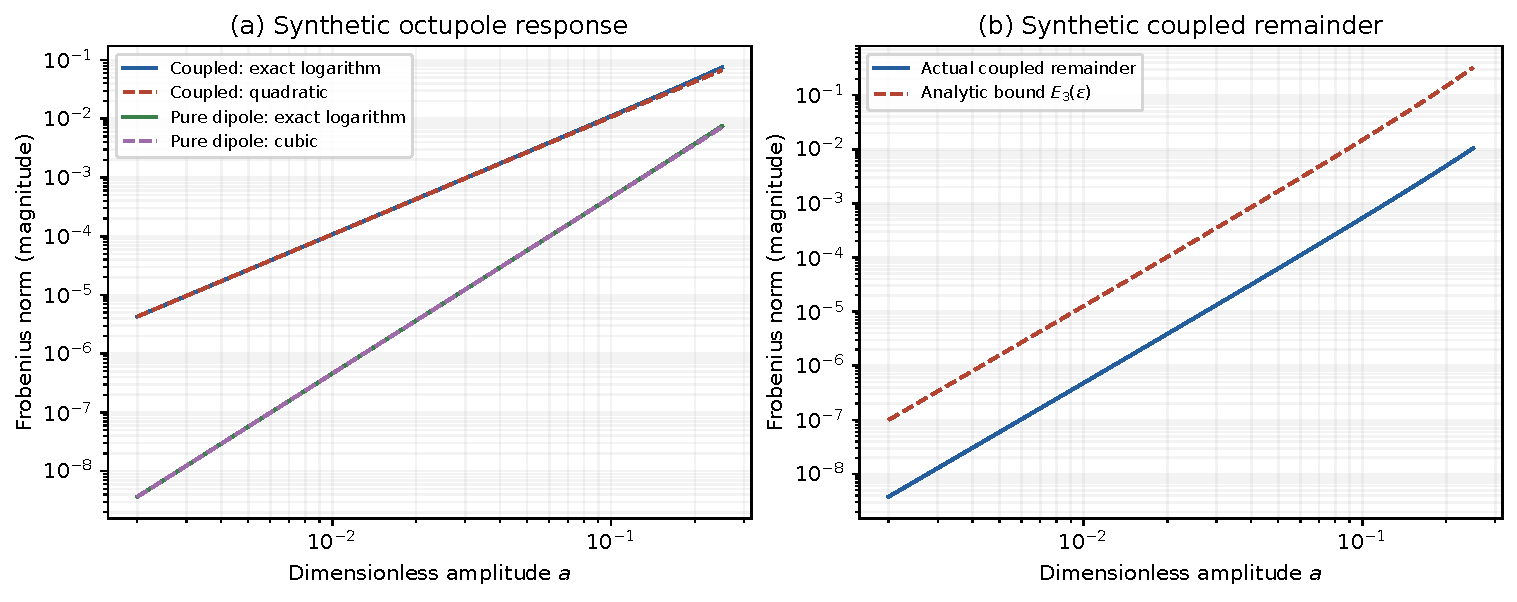
\includegraphics[width=\linewidth]{figures/optical.pdf}
\caption{Nonlinear local magnitude response for the specified synthetic acceleration and shear. The coupled octupole is quadratic at small common amplitude, whereas the pure-dipole response begins at cubic order. The right panel compares the saved exact-logarithm projection error with its analytic finite angular envelope. Curves consume the retained 45-row quadrature result; finite-redshift propagation and observational errors are separate inputs. All norm ordinates are in magnitude units; amplitude is dimensionless, and the response uses the same source and observer congruence.}\label{fig:optical}
\end{figure}
\begin{table}[htb]
\caption{Five retained synthetic local-response amplitudes. The amplitude $a$ is dimensionless; all other entries are full ordered-index Frobenius norms in magnitude units. The remainder is relative to the quadratic coupling, and the bound is $E_3(1.6a)$.}\label{tab:optical}
\begin{ruledtabular}
\begin{tabular}{ccccc}
$a$ & Exact coupled & Quadratic & Remainder & Bound \\
$2.00000\times10^{-3}$ & $4.28078\times10^{-6}$ & $4.27877\times10^{-6}$ & $3.79883\times10^{-9}$ & $9.95392\times10^{-8}$ \\
$6.68740\times10^{-3}$ & $4.79141\times10^{-5}$ & $4.78381\times10^{-5}$ & $1.42766\times10^{-7}$ & $3.74935\times10^{-6}$ \\
$2.23607\times10^{-2}$ & $5.37830\times10^{-4}$ & $5.34847\times10^{-4}$ & $5.43409\times10^{-6}$ & $1.43810\times10^{-4}$ \\
$7.47674\times10^{-2}$ & $6.10973\times10^{-3}$ & $5.97977\times10^{-3}$ & $2.16538\times10^{-4}$ & $5.88821\times10^{-3}$ \\
$2.50000\times10^{-1}$ & $7.44586\times10^{-2}$ & $6.68558\times10^{-2}$ & $1.04112\times10^{-2}$ & $3.22984\times10^{-1}$ \\
\end{tabular}\end{ruledtabular}\end{table}


The theorem, response and inverse concern a retained tensor carrier. In an application, we retain the common state \(Z\), its support and error region before forming scalar summaries. For the optical construction, a suitable deterministic carrier is \(x_\phi(Z)=(d,S,O_\mu,O_{\mu,\perp})\), with the shear contribution \(\Sigma_u^2=(S:S)/6\). At fixed known \(S\ne0\), a justified observational octupole error radius \(e_O\) gives the policy score

\begin{equation}
 Q_{\rm cpl}=\frac{\|\widehat O_{\mu,\perp}\|_F}
                         {E_3(\epsilon)+e_O}.
 \tag{41}
\end{equation}

The denominator is required to be positive; a zero denominator is handled as the exact constraint \(\widehat O_{\mu,\perp}=0\), without assigning a ratio. Uncertain shear requires the image over the joint admissible state region. A single best-fit eigenframe does not retain that dependence.

For a declared support measure \(\nu\) on an application domain \(D\), an occupancy can be defined as \(F_\nu(B)=\nu(B\cap D)/\nu(D)\), provided \(0<\nu(D)<\infty\). The occupied set \(B\), and any admissible physical ceiling used to define it, belong to that policy. A threshold exceedance \(\Pi_P(t)=P\{Q_{\rm cpl}(Z)>t\}\) additionally requires a named joint law \(P\). A depth comparison \(G_F\) requires registered windows and a specified functional of their \(F\) values, retaining shared calibration and cross-window dependence. The present synthetic family specifies neither such a sampling law nor an observational occupancy measure or depth functional, so these sectors remain undefined. Its deterministic \(x_\phi\), \(\mathcal C\) and response bounds do not supply them.

The local slope does not determine vorticity, curvature or a matter-frame energy split. Consequently the shear contribution alone cannot fill the other sectors of a signed physical comparator \(x\). Likewise, a temperature or polarization tensor pair requires its own transfer, mask and noise response before the optical interpretation can be applied. These requirements specify the measurements needed for a physical application; they do not enter the proof of the tensor inequality.

\section{Discussion}

The contraction \(O:Q\) reduces seven octupole components to three, but its lost information has a simple exact form. A four-dimensional affine kernel remains, and a norm constraint turns its interior fibres into three-spheres. The ellipsoid boundary selects a unique minimum-norm tensor. Balancing the three normalized contraction components then gives the fixed-quadrupole chirality maximum; a zero cubic trace of the quadrupole gives the sharp global constant.

The local distance response provides an interpretation of that boundary lift. Acceleration and shear enter the directional rate at first order, and their product generates a constrained octupole after the logarithmic magnitude conversion. Its complementary four components provide a residual morphology test, with a finite angular bound and a constructive inverse. The complete ideal field supplies an intercept-independent inverse, while an explicit small-amplitude family approaches both algebraic chirality endpoints.

These results organize amplitude, shape and response before a statistical law is introduced. An observational use can pass a joint tensor region through the same maps, with its finite-redshift, frame and calibration response retained. That preserves the information required to ask whether a measured higher multipole has the shape of a specified physical coupling.

\bibliographystyle{apsrev4-2}\bibliography{references}
\end{document}
